\section{Idea Behind Indexing}

Suppose you have a textbook and you want to look for a certain term, say, the word ``\textit{string}''. It would be really time-consuming, and in some cases, impossible to look for the term by going through the book page by page. That's why most books usually (and hopefully) have an index at the end, which list the pages where each term occurs.

\begin{figure}
    \centering
    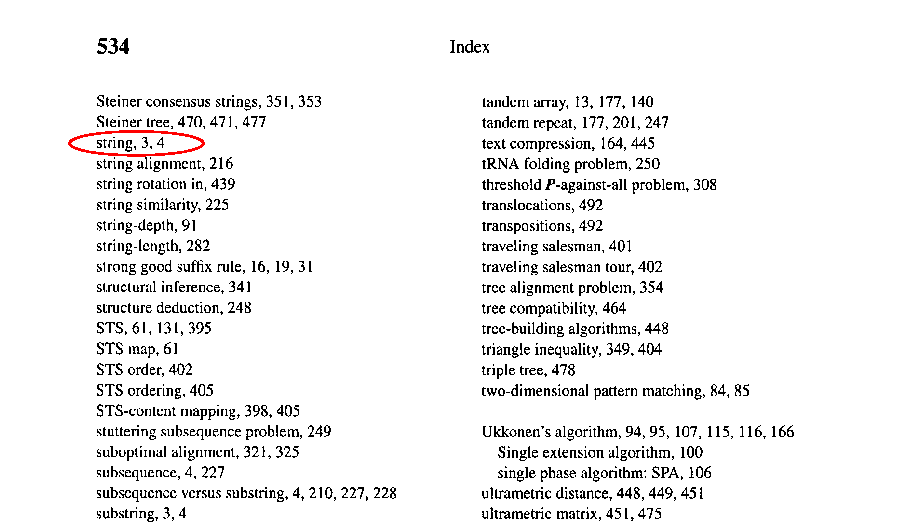
\includegraphics[width=\linewidth]{index/example-gusfield-idx.pdf}
    \label{fig:example-gusfield-idx}
    \caption{The index of Gusfield's textbook, with the term ``string'' circled.}
\end{figure}

Index can help us speed up query speed and also give us a compact representation of the data.

Two big ideas behind indexing are \textit{\textbf{grouping}} and \textit{\textbf{ordering}}. The first index that we will look at, $k$-mer index, uses grouping.

\section{\textit{k}-mer Index}

Given a text $T$, we call all its substrings of length $k$, the \textit{\textbf{k-mers}} of $T$. For example, consider the string \texttt{CGTGCGTGCTT}, it has the following 5-mers: \texttt{CGTGC}, \texttt{GCGTG}, \texttt{GTGCC}, \texttt{GTGCT}, \texttt{TGCCT}, and \texttt{TGCTT}. The substrings \textit{can have overlaps}.

$k$-mer index groups the indices of $T$ by the $k$-mer that starts at the index. So, for the string \texttt{CGTGCGTGCTT}, we have the $k$-mer index for $k=5$:

\begin{table}
    \centering
    \begin{tabular}[H]{c|c}
        $k$-mer & indices \\
        \hline
        \texttt{CGTGC} & 0, 4 \\
        \texttt{GCGTG} & 3 \\
        \texttt{GTGCC} & 1 \\
        \texttt{GTGCT} & 5 \\
        \texttt{TGCCT} & 2 \\
        \texttt{TGCTT} & 6
    \end{tabular}
\end{table}

It is easy to construct a $k$-mer index. We can scan the string from left to right and record the position of each $k$-mer. It takes $|T|-k+1$ time.

\section{Querying k-mer Index}

To query a $k$-mer index efficiently, we should first \textit{sort the index lexicographically} by the $k$-mers. It takes $k(|T|-k)\log(|T|-k) \in O(|T|^2 \log|T|)$ steps. To compare two $k$-mers, we need $k$ steps (unlike comparing two numbers or characters, which takes constant time), and sorting the list of $|T|-k$ $k$-mers takes $\Theta((|T|-k)\log(|T|-k))$. There is a bit of tradeoff here. If we choose a small $k$, we spend less time comparing two substrings during sorting, but we can possibly end with many $k$-mers in the list; in we choose a large $k$, it takes more time to compare two substrings, but we will have fewer $k$-mers to sort.

Once we sort the $k$-mer index, we can use \textit{binary search} for patterns $P$ such that $|P| \leq k$. It takes $O(|P|\log |T|)$ to query a sorted $k$-mer index. However, if $|P| > k$, $k$-mer index can be inefficient since we need to \textit{manually extend the match} once the first $k$ characters of $P$ matches a substring in $T$.